The \acf{MPI} library has about 250 routines, many of which you may
never need. Since this is a textbook, not a reference manual, we will
focus on the important concepts and give the important routines for
each concept. What you learn here should be enough for most common
purposes, but you are advised to keep a reference document handy, in
case there is a specialized routine, just for you.

\Level 0 {Basic concepts}

\Level 1 {Initialization / finalization}

Every program that uses MPI needs to initialize and finalize exactly
once. In~C, the calls are
\begin{verbatim}
ierr = MPI_Init(&argc,&argv);
// your code
ierr = MPI_Finalize();
\end{verbatim}
where \n{argc} and \n{argv} are the arguments of the main program.
%
The corresponding Fortran calls are
\begin{verbatim}
call MPI_Init(ierr)
// your code
call MPI_Finalize()
\end{verbatim}

We make a few observations.
\begin{itemize}
\item MPI routines return an error code. In~C, this is a function
  result; in Fortran it is the final parameter in the calling
  sequence.
\item For most routines, this parameter is the only difference between
  the C and Fortran calling sequence, but some routines differ in some
  respect related to the languages. In this case, C~has a mechanism
  for dealing with commandline arguments that Fortran lacks.
\item This error parameter is zero if the routine completes
  succesfully, and nonzero otherwise. You can write code to deal with
  the case of failure, but by default your program will simply abort
  on any MPI error. See section~\ref{mpi:error} for more details.
\end{itemize}

The commandline arguments \n{argc} and \n{argv} are only guaranteed to
be passed to process zero, so the best way to pass commandline information
is by a broadcast (section~\ref{sec:bcast}).

\Level 1 {Running an MPI program}

MPI programs can be run on many different architectures. Obviously it
is your ambition (or at least your dream) to run your code on a
cluster with a hundred thousand processors and a fast network. But
maybe you only have a small cluster with
plain \indexterm{ethernet}. Or maybe you're sitting in a plane, with
just your laptop. An MPI program can be run in all these
circumstances~--~within the limits of your available memory of course.

The way this works is that you do not start your executable directly,
but you use a program, typically called \n{mpirun}\index{mpirun} or
something similar, which makes a connection to all available
processors and starts a run of your executable there. So if you have a
thousand nodes in your cluster, \n{mpirun} can start your program once
on each, and if you only have your laptop it can start a few instances
there. In the latter case you will of course not get great
performance, but at least you can test your code for correctness.

\Level 1 {Distinguishing between processes}

In the SPMD model you run the same executable on each of a set of processors; see section~\HPSCref{sec:spmd}. So how can you do anything useful if all processors run the same code? Here is where your first two MPI routines come in.

With \indexmpi{MPI\_Comm\_size} a processor can query how many
processes there are in total, and with \indexmpi{MPI\_Comm\_rank} it
can find out what its number is. This rank is a number from zero to
the comm size minus~one. (Zero-based indexing is used even if you
program in Fortran.)

\begin{exercise}
  \label{ex:hello-world-zero}
  Write your first MPI program: make calls to \n{MPI_Comm_size} and
  \n{MPI_Comm_rank}, and let processor zero print out how many
  processes there are.

  Now alter your program so that, for instance, processor~5 prints
  `Hello, I~am processor 5~out of~12', et cetera. You will most likely
  see that the output does not appear on your screen (or in your log
  file if you run in batch mode) in sequence, or even nicely
  separated. We will fix this later.
\end{exercise}

\Level 0 {Point-to-point communication}

MPI has two types of message passing routines: point-to-point and
collectives. In this section we will discuss point-to-point
communication, which involves the interaction of a unique sender and a
unique receiver. Collectives, which involve all processes in some
joint fashion, will be discussed in the next section.

There is a lot to be said about simple sending and receiving of
data. We will go into three broad categories of operations: blocking
and non-blocking two-sided communication, and the somewhat
more tricky one-sided communication.

\Level 1 {Blocking communication}
\index{two-sided communication|(}
\index{blocking communication|(}

In two-sided communication, one process issues a send call and the
other a receive call. Life would be easy if the send call put the data
somewhere in the network for the receiving process to find whenever it
gets around to its receive call. This ideal scenario is pictured
figure~\ref{fig:send-ideal}.
\begin{figure}[ht]
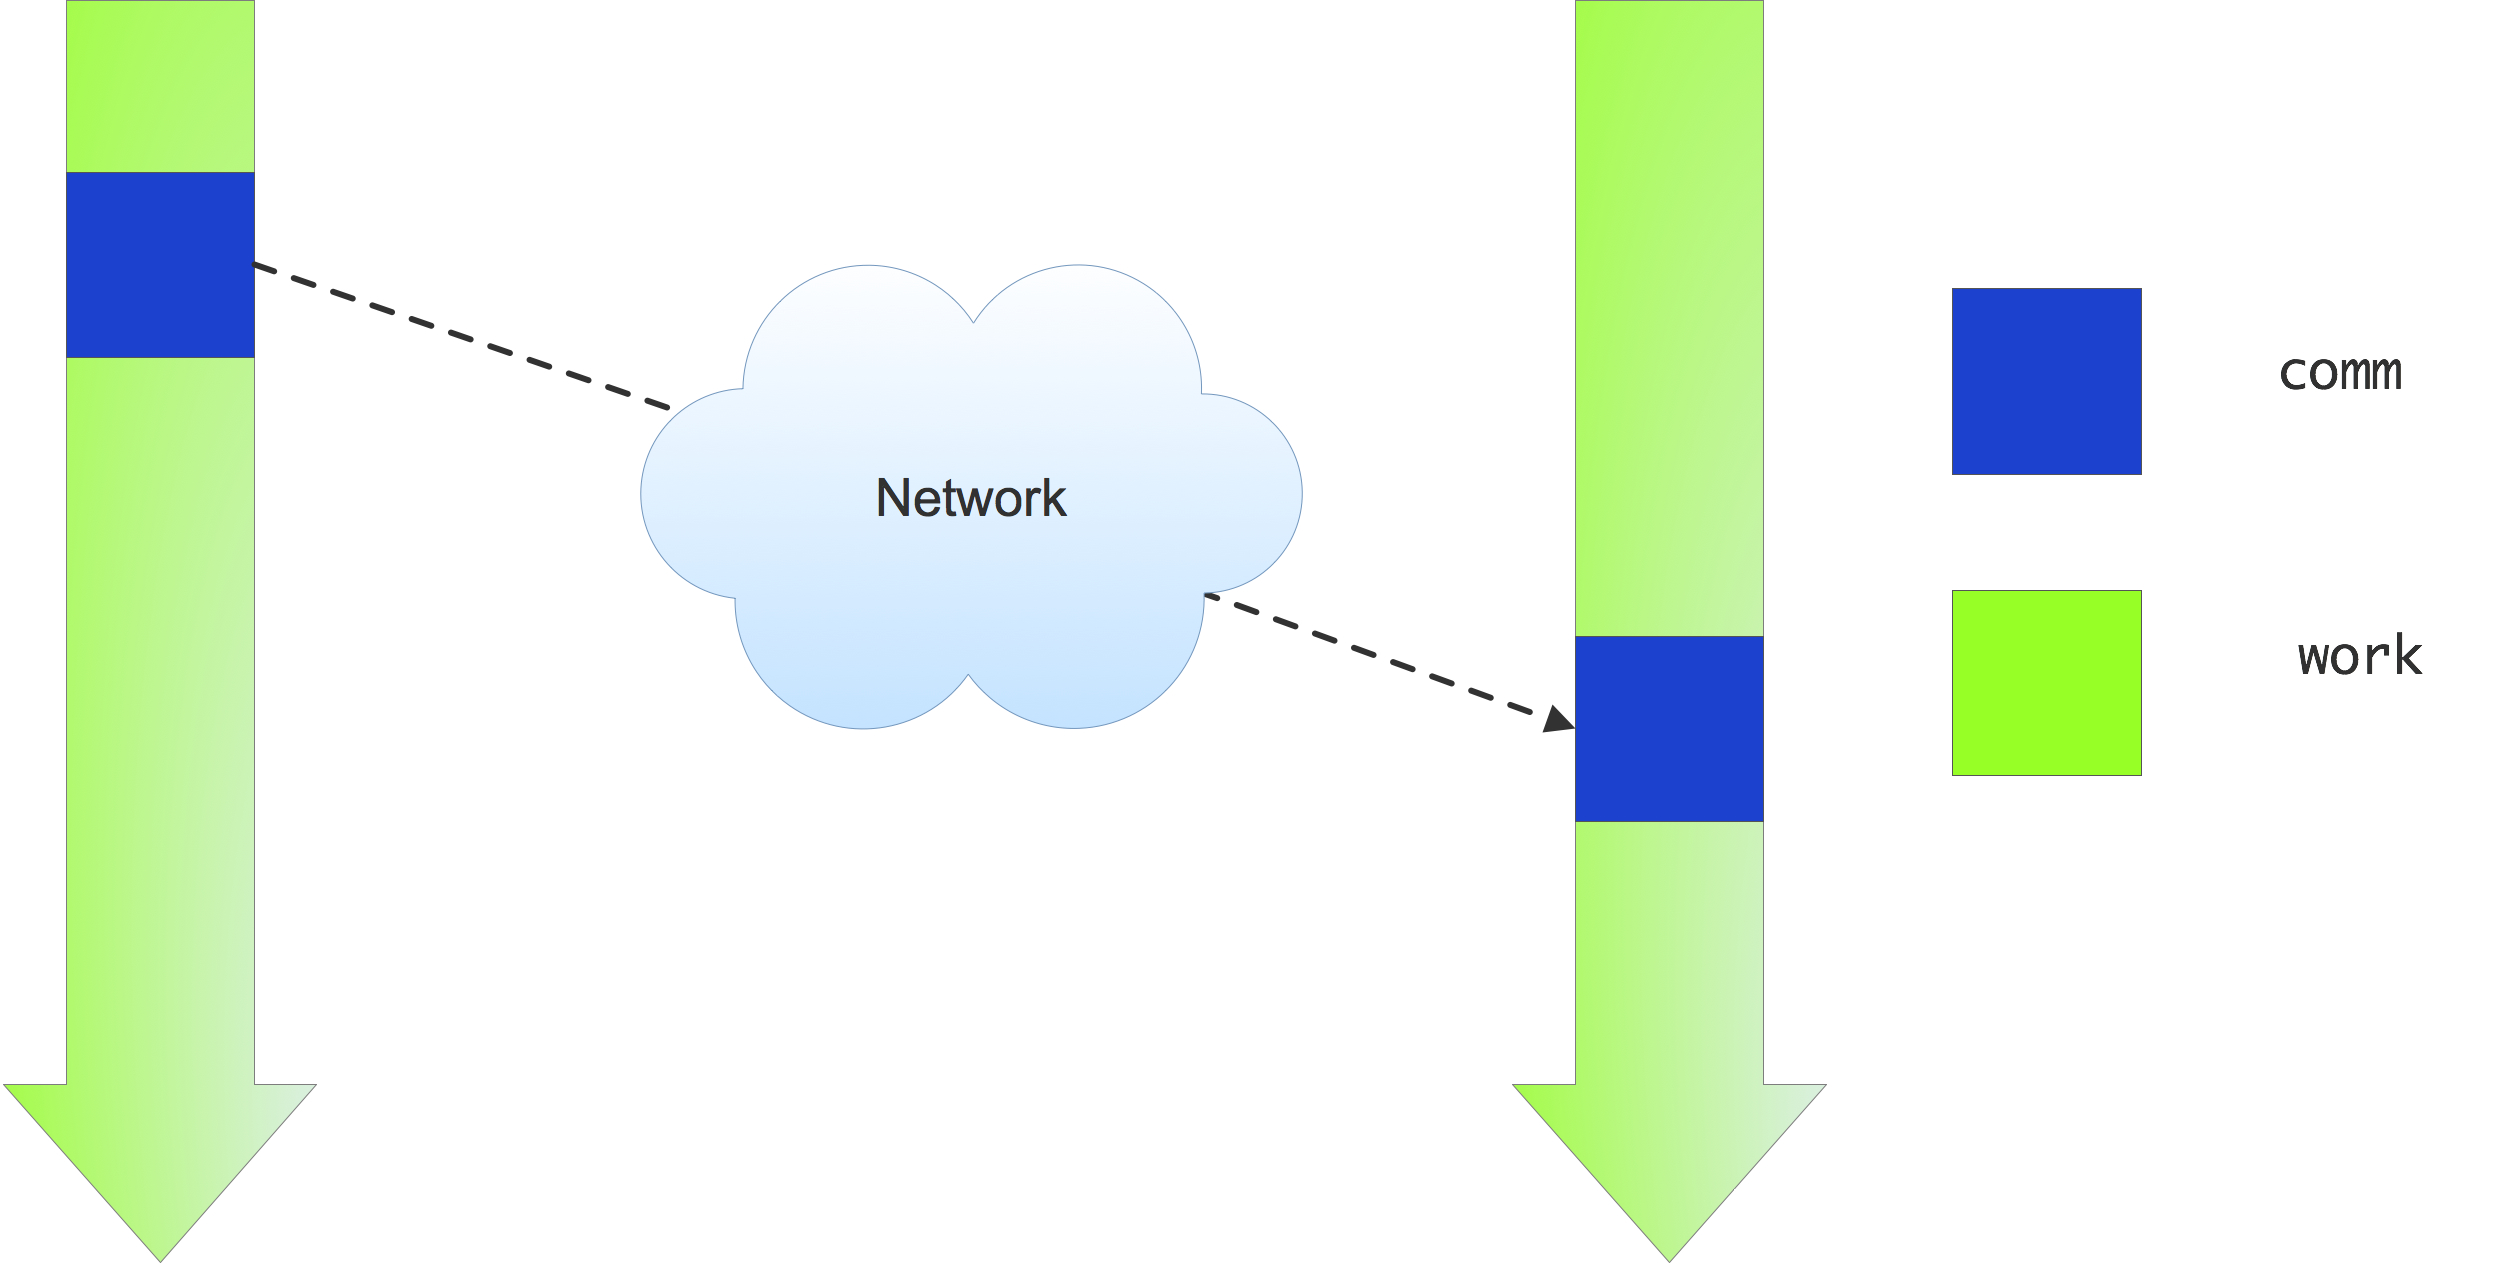
\includegraphics[scale=.1]{graphics-public/send-ideal}
\caption{Illustration of an ideal send-receive interaction}
\label{fig:send-ideal}
\end{figure}
Of course, if the receiving process gets to the receive call before
the send call has been issued, it will be idle until that happens.

Even if processes are optimally synchronized communication introduces
some overhead: there is an inital latency connected with every
message, and the network also has a limited bandwidth which leads to a
transfer time per byte; see~\HPSCref{sec:bwlatency}.

The above ideal scenario is not realistic: it assumes that somewhere
in the network there is buffer capacity for all messages that are in
transit. Since this message volume can be large, we have to worry
explicitly about management of send and receive \indexterm{buffers}.

The easiest scenario is that the sending process keeps the message
data in its address space until the receiving process has indicated
that it is ready to receive it. This is pictured in
figure~\ref{fig:send-blocking}.
\begin{figure}[ht]
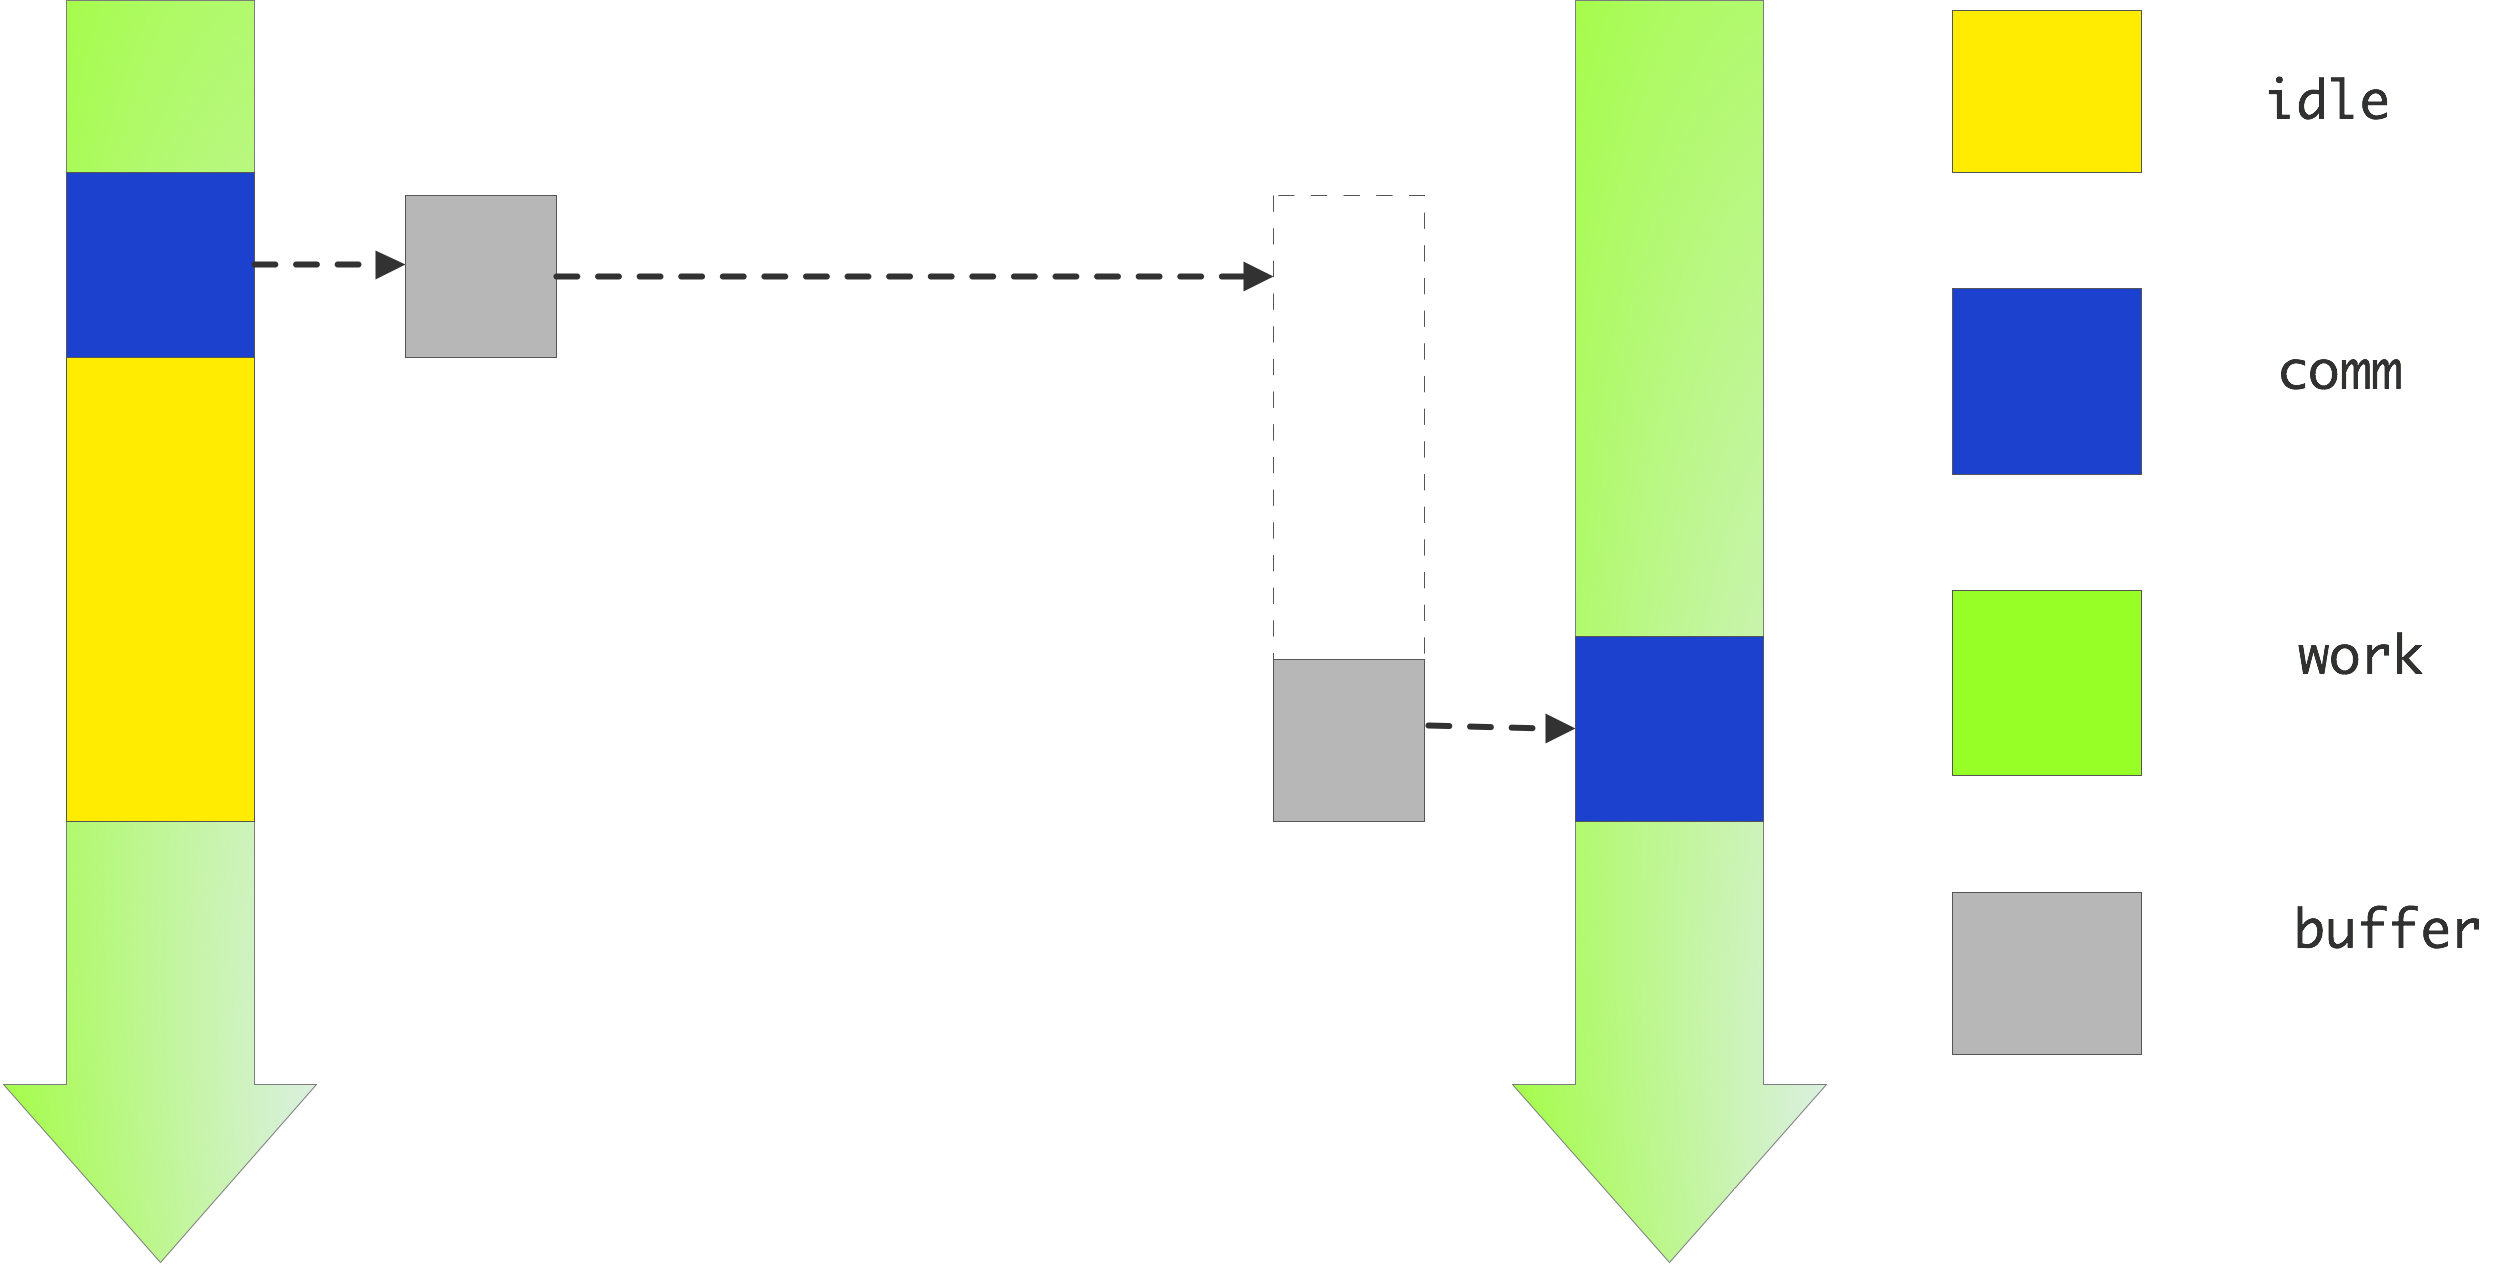
\includegraphics[scale=.1]{graphics-public/send-blocking}
\caption{Illustration of a blocking communication: the sending processor is idle until the receiving processor issues and finishes the receive call}
\label{fig:send-blocking}
\end{figure}
This is known as \emph{blocking} communication: a process that issues
a send or receive call will then block until the corresponding receive
or send call is successfully concluded.

It is clear what the first problem with this scenario is: if your
processes are not perfectly synchronized your performance may degrade
because processes spend time waiting for each other;
see~\HPSCref{sec:load}. 

But there is a more insidious, more serious problem.
Suppose two process need to exchange data, and consider the following
pseudo-code, which purports to exchange data between processes 0 and~1:
\begin{verbatim}
other = 1-mytid; /* if I am 0, other is 1; and vice versa */
send(target=other);
receive(source=other);
\end{verbatim}
Imagine that the two processes execute this code. They both issue the
send call\ldots\ and then can't go on, because they are both waiting
for the other to issue a receive call. This is known
as \indexterm{deadlock}.

The solution is to first do the send from 0 to~1, and then from 1 to~0 (or the other way around). So the code would look like:
\begin{verbatim}
if ( /* I am processor 0 */ ) {
  send(target=other);
  receive(source=other);
} else {
  receive(source=other);
  send(target=other);
}
\end{verbatim}

There is even a third, even more subtle problem with blocking
communication. Consider the scenario where every processor needs to
pass data to its successor, that is, the processor with the next
higher rank. The basic idea would be to first send to your successor,
then receive from your predecessor. Since the last processor does not
have a successor it skips the send, and likewise the first processor
skips the receive. The pseudo-code looks like:
\begin{verbatim}
successor = mytid+1; predecessor = mytid-1;
if ( /* I am not the last processor */ )
  send(target=successor);
if ( /* I am not the first processor */ )
  receive(source=predecessor)
\end{verbatim}
This code does not deadlock. All processors but the last one block on
the send call, but the last processor executes the receive call. Thus,
the processor before the last one can do its send, and subsequently
continue to its receive, which enables another send, et cetera.

Thus, this code will terminate (instead of hanging forever on a
deadlock) and do what you intended it to do. However, the execution
now suffers from \indextermsub{unexpected}{sequentialization}: only
one processor is active at any time, so what should have been a
parallel operation becomes a sequential one.

\begin{exercise}
  Give pseudo-code for a solution that uses blocking operations, and is
  parallel --~although maybe not optimally so.
\end{exercise}

It is possible to orchestrate your processes to get an efficient and
deadlock-free execution, but there are better solutions which we will
now explore.

\begin{exercise}
  There are rare circumstances where you actually want this serial
  behaviour. Recall from exercise~\ref{ex:hello-world-zero} that
  output from processes is not automatically serialized. Take your
  code from that exercise, and use the serialization behaviour your
  observed to force the processes to output their print statements in
  sequence.
\end{exercise}

\Level 2 {Blocking and small messages}

Blocking communication involves a complicated dialog between the two
processors involved. Processor one says `I~have this much data to
send; do you have space for that?', to which processor two replies
`yes, I~do; go ahead and send', upon which processor one does the
actual send. This back-and-forth (technically known as
a \indexterm{handshake}) takes a certain amount of communication
overhead. For this reason, network hardware will sometimes forgo the
handshake for small messages, and just send them regardless, knowing
that the other process has a small buffer for such occasions.

One strange side-effect of this strategy is that a code that
should \indexterm{deadlock} according to the MPI specification does
not do so. In effect, you may be shielded from you own programming
mistake! Of course, if you then run a larger problem, and the small
message becomes larger than the threshold, the deadlock will suddenly
occur. So you find yourself in the situation that a bug only manifests
itself on large problems, which are usually harder to debug. In this
case, replacing every \n{MPI_Send} with a \indexmpi{MPI\_Ssend} will force the
handshake, even for small messages.

\index{blocking communication|)}
\Level 1 {Non-blocking communication}
\index{non-blocking communication|(}

figure~\ref{fig:send-blocking}.
\begin{figure}[ht]
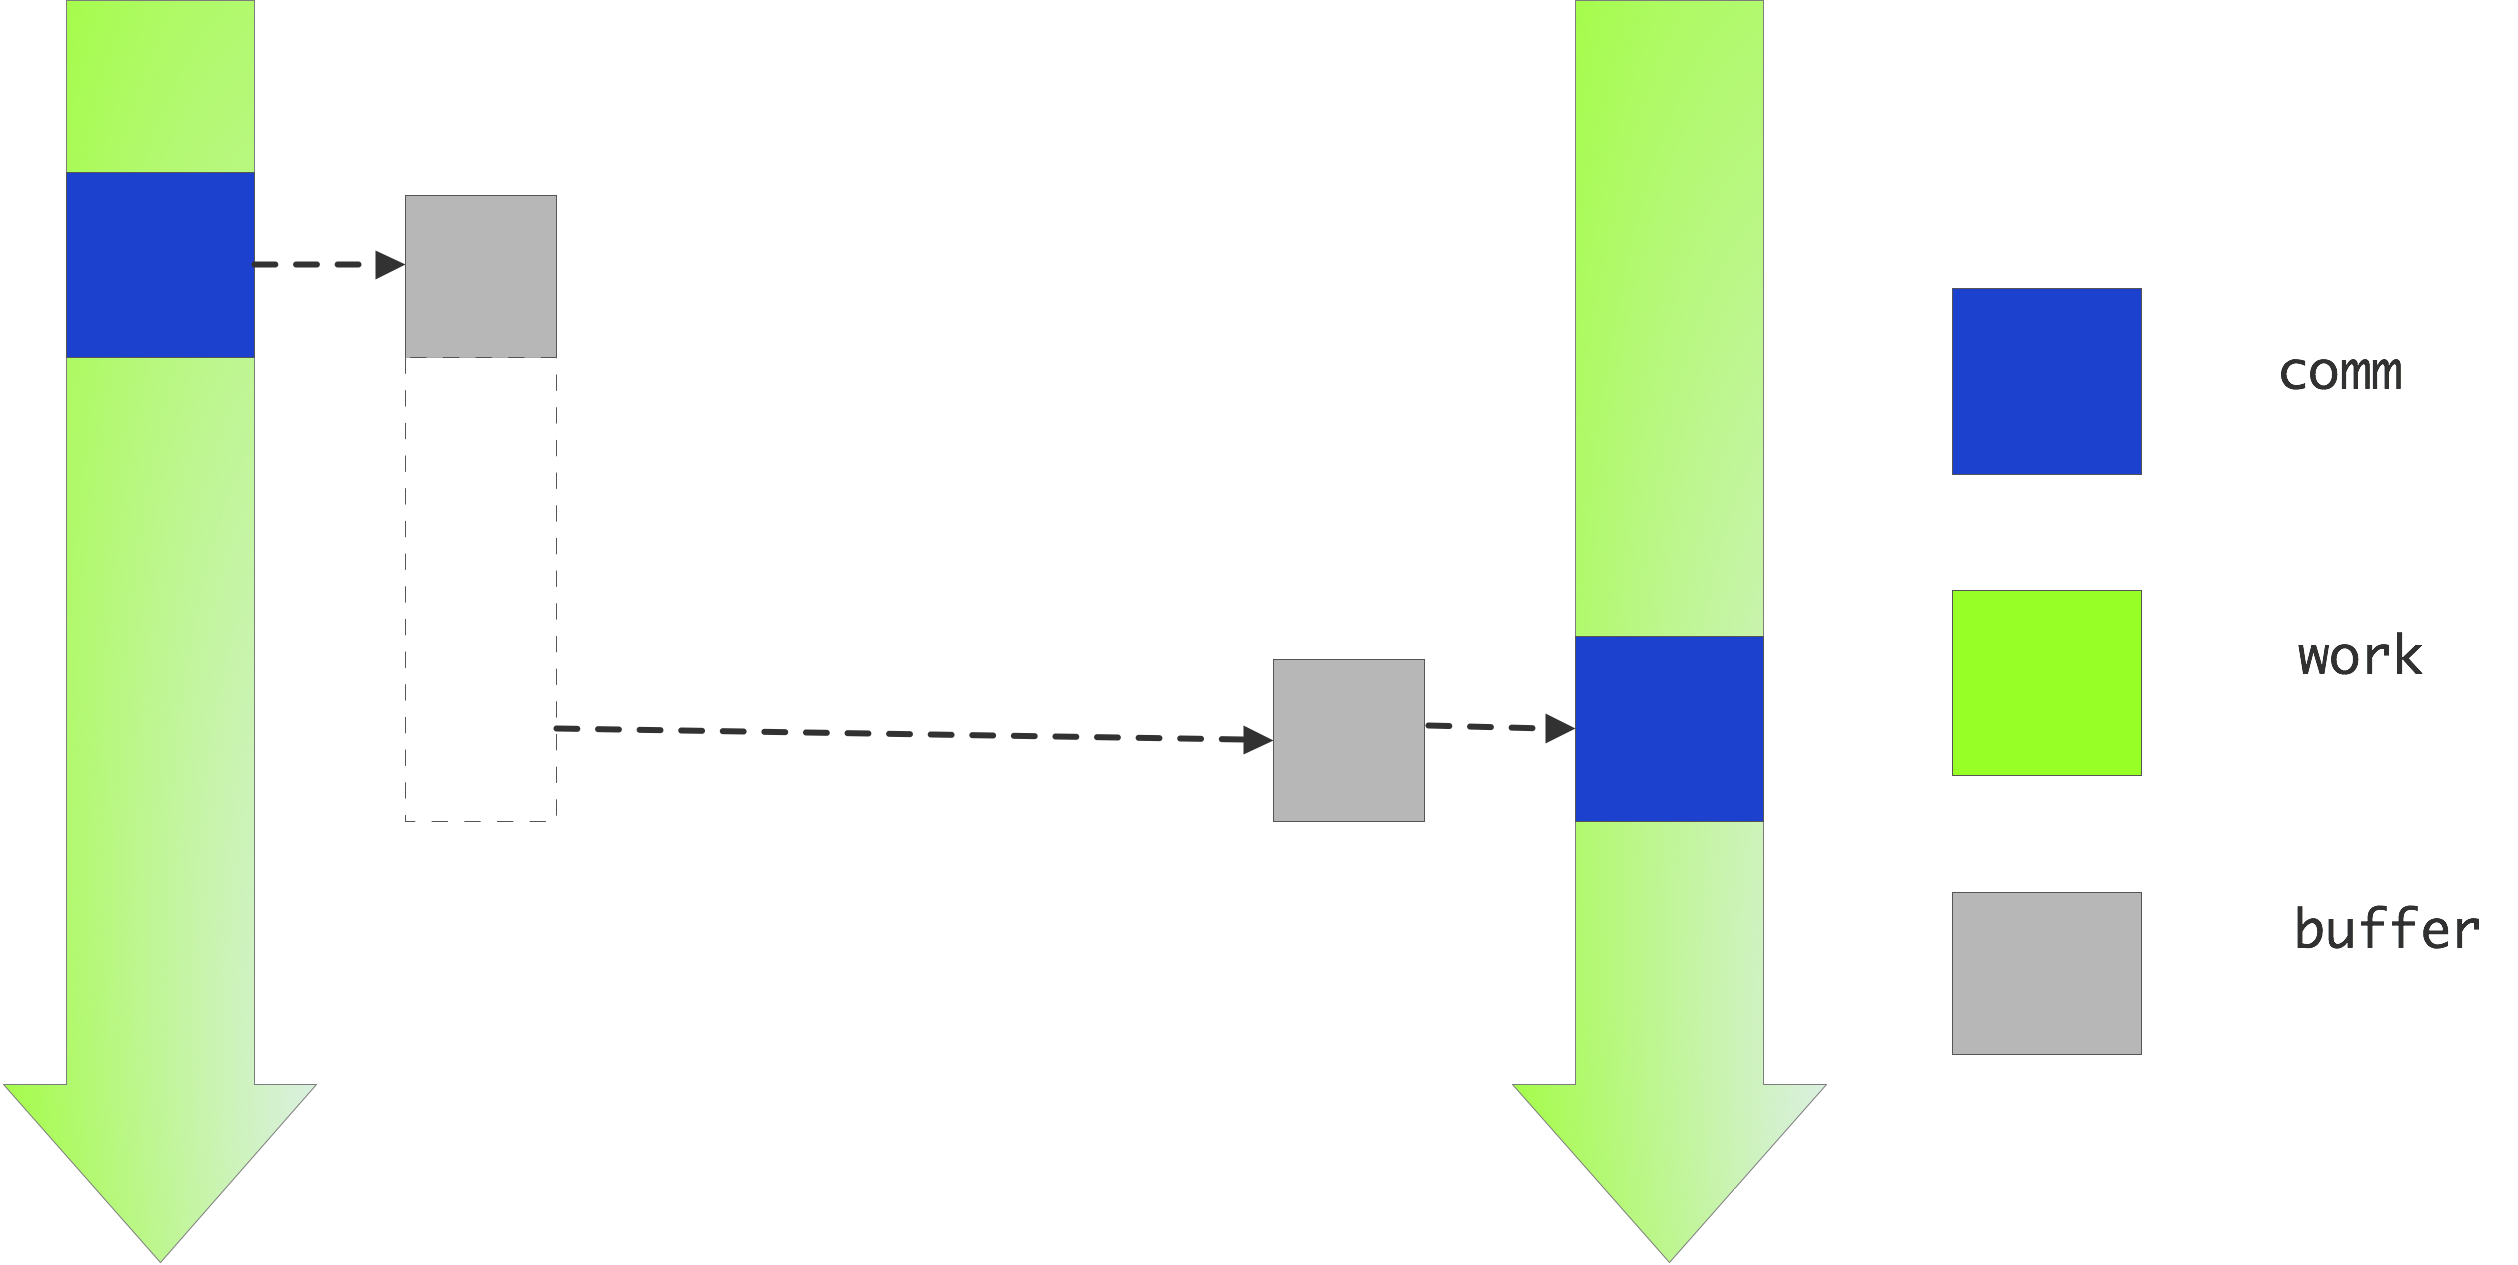
\includegraphics[scale=.1]{graphics-public/send-nonblocking}
\caption{Illustration of a non-blocking communication: the sending processor immediately continues execution after issueing the send call}
\label{fig:send-nonblocking}
\end{figure}

\index{non-blocking communication|)}
\index{two-sided communication|)}
\Level 1 {One-sided communication}
\index{one-sided communication|(}
\index{one-sided communication|)}

\Level 0 {Collectives}
\label{sec:bcast}

\Level 0 {Communicators}

A communicator is an object describing a group of processes. In many 
applications all processes work together closely coupled, and the
only communicator you need is \n{MPI_COMM_WORLD}. However, there are 
circumstances where you want one subset of processes to operate 
independently of another subset. For example:
\begin{itemize}
\item If processors are organized in a $2\times2$ grid, you may want
  to do broadcasts inside a row or column. 
\item For an application that includes a producer and a consumer part,
  it makes sense to split the processors accordingly.
\end{itemize}
In this section we will see mechanisms for defining new communicators
and sending messages between communicators.

\Level 1 {Intra-communicators}
\label{sec:comm-group}

We start by exploring the mechanisms for creating a communicator that
encompasses a subset of \n{MPI_COMM_WORLD}. 

There is a simple function that splits a communicator into disjoint
communicators:
\begin{verbatim}
MPI_COMM_SPLIT(MPI_Comm comm, int color, int key, MPI_Comm newcomm, ierr)
\end{verbatim}
Each processor specifies what `colour' it is, and processes with the
same colour are grouped into a joint communicator. The `key' value is
used to determine the rank in the new communicator.

The most general mechanism for creating communicators is through
process groups: you can query the group of processes of a
communicator, manipulate groups, and make a new communicator out of a
group you have formed.

\begin{verbatim}
MPI_COMM_GROUP (comm, group, ierr)
MPI_COMM_CREATE (MPI_Comm comm,MPI_Group group, MPI_Comm newcomm, ierr)
\end{verbatim}

\begin{verbatim}
MPI_GROUP_UNION(group1, group2, newgroup, ierr)
MPI_GROUP_INTERSECTION(group1, group2, newgroup, ierr)
MPI_GROUP_DIFFERENCE(group1, group2, newgroup, ierr)
\end{verbatim}

\begin{verbatim}
MPI_GROUP_INCL(group, n, ranks, newgroup, ierr)
MPI_GROUP_EXCL(group, n, ranks, newgroup, ierr)
\end{verbatim}
\begin{verbatim}
MPI_GROUP_SIZE(group, size, ierr)
MPI_GROUP_RANK(group, rank, ierr)
\end{verbatim}

\Level 1 {Inter-communicators}

If two disjoint communicators exist, it may be necessary to
communicate between them. This can of course be done by creating a new
communicator that overlaps them, but this would be complicated: since
the `inter' communication happens in the overlap communicator, you
have to translate its ordering into those of the two worker
communicators. It would be easier to express messages directly in
terms of those communicators, and this can be done with
`inter-communicators'.

\begin{verbatim}
MPI_INTERCOMM_CREATE (local_comm, local_leader, bridge_comm, remote_leader, tag, newintercomm, ierr)
\end{verbatim}
After this, the intercommunicator can be used in collectives such as
\begin{verbatim}
MPI_BCAST (buff, count, dtype, root, comm, ierr)
\end{verbatim}
\begin{itemize}
\item In group~A, the root process passes \n{MPI_ROOT} as
  `root' value; all others use \n{MPI_NULL_PROC}.
\item In group~B, all processes use a `root' value that is the
  rank of the root process in the root group.
\end{itemize}
Gather and scatter behave similarly; the allgather is different: all
send buffers of group~A are concatenated in rank order, and places on
all processes of group~B.

Inter-communicators can be used if two groups of process work
asynchronously with respect to each other; another application is
fault tolerance (section~\ref{mpi:tolerant}).

\Level 0 {One-sided communication}

Above, you saw collectives and point-to-point operations. The latter
type had in common that they require the co-operation of a sender and
receiver. This co-operation could be loose: you can post a receive
with \n{MPI_ANY_SOURCE} as sender, but there had to be both a send and
receive call. On the other hand, in one-sided communication a process
can do a `put' or `get' operation, writing data to or reading it from
another processor, without that other processor's involvement.

In one-sided MPI operations, also known as \acf{RMA} operations, there
are still two processes involved: the \indexterm{origin}, which is the
process that originates the transfer, whether this is a `put' or a `get',
and the \indexterm{target} whose
memory is being accessed. On the target, you declare an area of
user-space memory that is accessible to other processes. This is known
as a \indexterm{window}. Windows limit how origin processes can access
the target's memory: you can only `get' data from a window or `put' it
into a window; all the other memory is not reachable from other processes.

A window is a contiguous area of memory:
\begin{verbatim}
MPI_WIN_CREATE (void *base, MPI_Aint size, 
int disp_unit, MPI_Info info, MPI_Comm 
comm, MPI_Win *win, ierr)
\end{verbatim}
A window is defined with respect to a communicator: each process
specifies a memory area. (This routine is collective, so each
process \emph{has} to call this routine.) These areas are then
accessible to other processes in the communicator by specifying the
process rank and an offset from the base of the window.
\begin{verbatim}
MPI_PUT (void *origin_addr, int origin_count, MPI_Datatype 
origin_datatype, int target_rank, MPI_Aint target_disp, int 
target_count, MPI_Datatype target_datatype, MPI_Win 
window, ierr)
\end{verbatim}
The \n{MPI_Get} call is very similar; a third one-sided routine
is \n{MPI_Accumulate} which does a reduction operation on the results
that are being put:
\begin{verbatim}
MPI_ACCUMULATE (void *origin_addr, int
origin_count, MPI_Datatype origin_datatype, 
int target_rank, MPI_Aint target_disp, int
target_count, MPI_Datatype
target_datatype,MPI_Op op,MPI_Win 
window,ierr)
\end{verbatim}

With a two-sided operation it is clear when the message has been
completed; with a one-sided operation this is not so clear. Therefore
we need a mechanism to ensure successful completion. One possibility
is to use a \indexterm{fence}.
\begin{verbatim}
MPI_WIN_FENCE (int assert, MPI_Win win, ierr)
\end{verbatim}
This is comparable to doing a barrier on the communicator on which the
window was based, and it guarantees that all communication on the
window is completed.

A fence delineates a so-called \indexterm{epoch}. In fact, you
can put fences around the epoch, giving various hints to the system
through the \n{assert} parameter.
\begin{verbatim}
MPI_Win_fence((MPI_MODE_NOPUT | MPI_MODE_NOPRECEDE), win);
MPI_Get( /* operands */, win);
MPI_Win_fence(MPI_MODE_NOSUCCEED, win);
\end{verbatim}

\begin{exercise}
  Implement an `all-gather' operation using one-sided communication:
  each processor stores a single number, and you want each processor
  to build up an array that contains the values from all
  processors. Note that you do not need a special case for a processor
  collecting its own value: doing `communication' between a processor
  and itself is perfectly legal.
\end{exercise}

\Level 1 {Put vs Get}

\begin{verbatim}
while(!converged(A)){ 
  update(A); 
  MPI_Win_fence(MPI_MODE_NOPRECEDE, win); 
  for(i=0; i < toneighbors; i++) 
    MPI_Put(&frombuf[i], 1, fromtype[i], toneighbor[i], 
                         todisp[i], 1, totype[i], win); 
  MPI_Win_fence((MPI_MODE_NOSTORE | MPI_MODE_NOSUCCEED), win); 
  } 
\end{verbatim}
\begin{verbatim}
  while(!converged(A)){ 
  update_boundary(A); 
  MPI_Win_fence((MPI_MODE_NOPUT | MPI_MODE_NOPRECEDE), win); 
  for(i=0; i < fromneighbors; i++) 
    MPI_Get(&tobuf[i], 1, totype[i], fromneighbor[i], 
                    fromdisp[i], 1, fromtype[i], win); 
  update_core(A); 
  MPI_Win_fence(MPI_MODE_NOSUCCEED, win); 
  } 
\end{verbatim}

\Level 1 {Active and passive target synchronization}

There are two more fine-grained ways of doing one-sided communication
that are suitable if only a small number of processor pairs is
involved.  In \indexterm{active target synchronization} both
processors are involved through the calls \n{MPI_Win_start},
\n{MPI_Win_complete}, \n{MPI_ Win_post}, \n{Win_wait}. What routine
you use depends on whether the processor is an \indexterm{origin} or
\indexterm{target}.

If the current process is going to have the data in its window accessed,
you define an \indextermsub{exposure}{epoch} by:
\begin{verbatim}
MPI_Win_post( /* group of origin processes */ )
MPI_Win_wait()
\end{verbatim}
This turns the current processor into a target for access operations issued
by a different process.

If the current process is going to be issuing one-sided operations,
you define an \indextermsub{access}{epoch} by:
\begin{verbatim}
MPI_Win_start()
MPI_Win_complete()
\end{verbatim}
This turns the current process into the origin of a number of
one-sided access operations.

The `post' and `start' routines open the window to a
\indextermbus{group of}{processors}; see section~\ref{sec:comm-group}
for how to get such a group from a communicator.

In \indexterm{passive target synchronization} only one processor
is involved in the communication. This involves using
a lock: one process can lock the window
on another, specified, process.
\begin{verbatim}
MPI_WIN_LOCK (int locktype, int rank, int assert, MPI_Win win,ierr)
MPI_WIN_UNLOCK (int rank, MPI_Win win, ierr)
\end{verbatim}
During an access epoch, a process can initiate and finish a one-sided
transfer.
\begin{verbatim}
If (rank == 0) {
  MPI_Win_lock (MPI_LOCK_SHARED, 1, 0, win);
  MPI_Put (outbuf, n, MPI_INT, 1, 0, n, MPI_INT, win);
  MPI_Win_unlock (1, win);
}
\end{verbatim}
These routines make MPI behave like a shared memory system; the
instructions between locking and unlocking the window effectively
become \indexterm{atomic operations}.

\Level 1 {Details}

Sometimes an architecture has memory that is shared between processes,
or that otherwise is fast for one-sided communication. To put a window
in such memory, it can be placed in memory that is especially
allocated:
\begin{verbatim}
MPI_Alloc_mem() and MPI_Free_mem()
\end{verbatim}
These calls reduce to \n{malloc} and \n{free} is there is no special
memory area.

\Level 0 {Leftover topics}

\Level 1 {Status object}

The \n{MPI_Status} object is a structure with the following 
freely accessible members:
\n{MPI_SOURCE}, \n{MPI_TAG}, and \n{MPI_ERROR}. There is also opaque 
information: the amount of data received can be retrieved by 
a function call to \n{MPI_Get_count}.
\begin{verbatim}
int MPI_Get_count(
  MPI_Status *status,
  MPI_Datatype datatype,
  int *count
);
\end{verbatim}
This may be necessary since the \n{count} argument to \n{MPI_Recv} is 
the buffer size, not an indication of the actually expected number of
data items.

\Level 1 {Error handling}
\label{mpi:error}

Errors in normal programs can be tricky to deal with; errors in
parallel programs can be even harder. This is because in addition to
everything that can go wrong with a single executable (floating point
errors, memory violation) you now get errors that come from faulty
interaction between multiple executables.

A few examples of what can go wrong:
\begin{itemize}
\item MPI errors: an MPI routine can abort for various reasons, such
  as receiving much more data than its buffer can accomodate. Such
  errors, as well as the more common type mentioned above, typically
  cause your whole execution to abort. That is, if one incarnation of
  your executable aborts, the MPI runtime will kill all others.
\item Deadlocks and other hanging executions: there are various
  scenarios where your processes individually do not abort, but are all
  waiting for each other. This can happen if two processes are both
  waiting for a message from each other, and this can be helped by
  using non-blocking calls. In another scenario, through an error in
  program logic, one process will be waiting for more messages
  (including non-blocking ones) than are sent to it.
\end{itemize}

The MPI library has a general mechanism for dealing with errors that
it detects. The default behaviour, where the full run is aborted, is
equivalent to your code having the following statement\footnote{The
  routine \n{MPI\_Errhandler\_set} is deprecated.}  :
\begin{verbatim}
MPI_Comm_set_errhandler(MPI_COMM_WORLD,MPI_ERRORS_ARE_FATAL);
\end{verbatim}
Another simple possibility is to specify
\begin{verbatim}
MPI_Comm_set_errhandler(MPI_COMM_WORLD,MPI_ERRORS_RETURN);
\end{verbatim}
which gives you the opportunity to write code that handles the error
return value.

In most cases where an MPI error occurs a complete abort is the
sensible thing, since there are few ways to recover. The second
possibility can for instance be used to print out debugging
information:
\begin{verbatim}
ierr = MPI_Something();
if (ierr!=0) {
    // print out information about what your programming is doing
    MPI_Abort();
}
\end{verbatim}
One cases where errors can be handled is that of \emph{MPI file
  I/O}\indexterm{MPI!I/O}: if an output file has the wrong
permissions, code can possibly progress without writing data, or
writing to a temporary file.

\Level 1 {Fault tolerance}
\label{mpi:tolerant}

Processors are not completely reliable, so it may happen that one
`breaks': for software or hardware reasons it becomes
unresponsive. For an MPI program this means that it becomes impossible
to send data to it, and any collective operation involving it will
hang. Can we deal with this case? Yes, but it involves some
programming.

First of all, one of the possible MPI error return codes
(section~\ref{mpi:error}) is \n{MPI_ERR_COMM}, which can be returned
if a processor in the communicator is unavailable. You may want to
catch this error, and add a `replacement processor' to the
program. For this, the \n{MPI_Comm_spawn} can be used:
\begin{verbatim}
int MPI_Comm_spawn(char *command, char *argv[], int maxprocs, MPI_Info info, 
                  int root, MPI_Comm comm, MPI_Comm *intercomm,
                  int array_of_errcodes[])
\end{verbatim}
But this requires a change of program design: the communicator
containing the new process(es) is not part of the
old \n{MPI_COMM_WORLD}, so it is better to set up your code as a
collection of inter-communicators to begin with.

\Level 1 {Debugging}

There are various ways of debugging an MPI program. Typically there
are two cases. In the simple case your program can have a serious
error in logic which shows up even with small problems and a small
number of processors. In the more difficult case your program can only
be run on large scale, or the problem only shows up when you run at
large scale. For the second case you, unfortunately, need a dedicated
debugging tool, and of course the good ones are expensive. In the
first case there are some simpler solutions.

\Level 2 {Small scale debugging}

If your program hangs or crashes even with small numbers of
processors, you can try debugging on your local desktop or laptop
computer:
\begin{verbatim}
mpirun -np <n> xterm -e gdb yourprogram
\end{verbatim}
This starts up a number of X~terminals, each of which runs your
program. The magic of \n{mpirun} makes sure that they all collaborate
on a parallel execution of that program. If your program needs
commandline arguments, you have to type those in every xterm:
\begin{verbatim}
run <argument list>
\end{verbatim}
See appendix~\ref{tut:debug} for more about debugging with~\n{gdb}.

This approach is not guaranteed to work, since it depends on
your \n{ssh} setup; see the discussion
in \url{http://www.open-mpi.org/faq/?category=debugging#serial-debuggers}.

\Level 2 {Large scale debugging}

Check out \indexterm{ddt} or \indexterm{TotalView}.

\Level 2 {Memory debugging of MPI programs}

The commercial parallel debugging tools typically have a memory
debugger. For an open source solution you can
use \indexterm{valgrind}, but that requires some setup during
installation. See \url{http://valgrind.org/docs/manual/mc-manual.html#mc-manual.mpiwrap}
for details.

\Level 0 {A realistic programming example}

In this section we will gradually build a semi-realistic example
program. To get you started some pieces have already been written:
as a starting point look at \n{code/mpi/c/grid.cxx}.

\Level 1 {Description of the problem}

With this example you will investigate several strategies for
implementing a simple iterative method. Let's say you have a
two-dimensional grid of datapoints $G=\{g_{ij}\colon 0\leq
i<n_i,\,0\leq j<n_j\}$ and you want to compute~$G'$ where
\begin{equation}
g'_{ij} = 1/4 \cdot (g_{i+1,j}+g_{i-1,j}+g_{i,j+1}+g_{i,j-1}).
\label{eq:grid-update}
\end{equation}

This is easy enough to implement sequentially, but in parallel this
requires some care.

Let's divide the grid $G$ and divide it over a two-dimension grid of
$p_i\times p_j$
processors. (Other strategies exist, but this one scales best; see
section~\HPSCref{sec:pspmvp}.)
Formally, we define two sequences of points
\[ 0=i_0<\cdots<i_{p_i}<i_{p_i+1}=n_i,\quad 
   0<j_0<\cdots<j_{p_j}<i_{p_j+1}=n_j
\]
and we say that processor $(p,q)$ computes $g_{ij}$ for
\[ i_p\leq i<i_{p+1}, \quad j_q\leq j<j_{q+1}.
\]
From formula~\eqref{eq:grid-update} you see that the processor then
needs one row of points on each side surrounding its part of the
grid. A~picture makes this clear; see figure~\ref{fig:ghost-grid}.
\begin{figure}
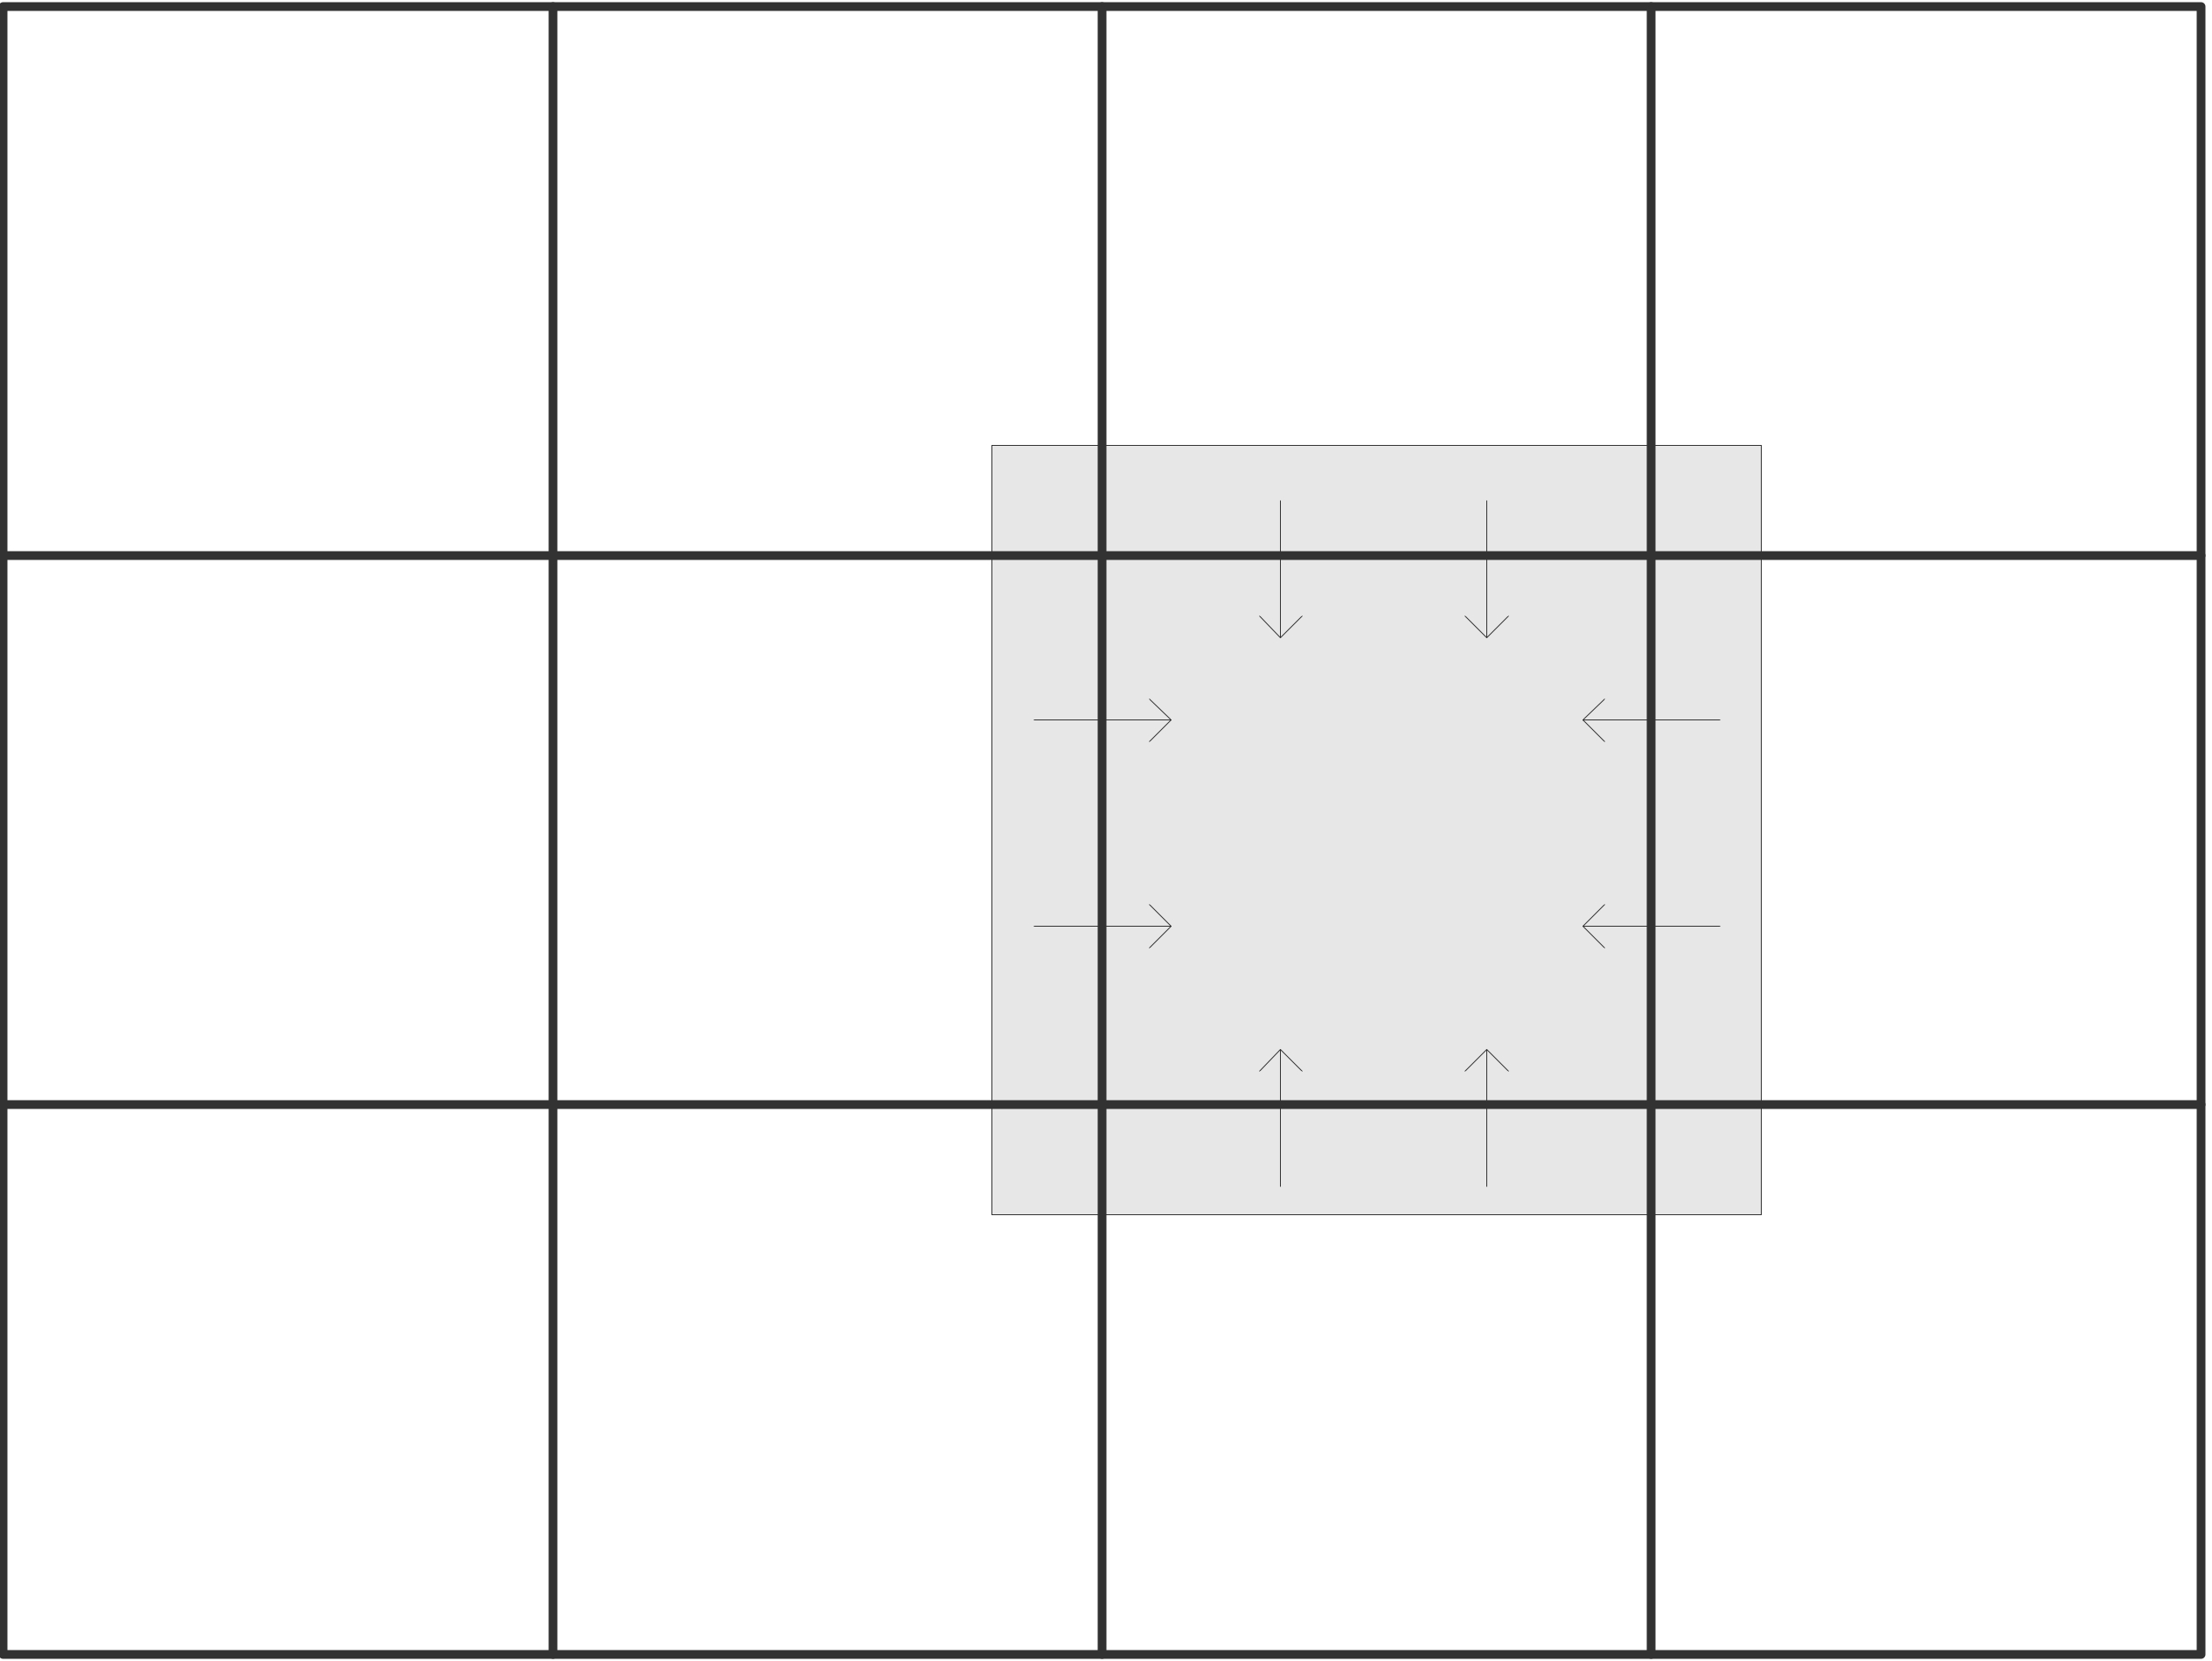
\includegraphics[scale=.1]{graphics-public/jacobi-average}
\caption{A grid divided over processors, with the `ghost' region indicated}
\label{fig:ghost-grid}
\end{figure}
These elements surrounding the processor's own part are called
the \indexterm{halo} or \indexterm{ghost region} of that processor.

The problem is now that the elements in the halo are stored on a
different processor, so communication is needed to gather them. In the
upcoming exercises you will have to use different strategies for doing
so.

\Level 1 {Code basics}

The program needs to read the values of the grid size and the
processor grid size from the commandline, as well as the number of
iterations. This routine does some error checking: if the number of
processors does not add up to the size of \n{MPI_COMM_WORLD}, a
nonzero error code is returned.
\begin{verbatim}
ierr = parameters_from_commandline
  (argc,argv,comm,&ni,&nj,&pi,&pj,&nit);
if (ierr) return MPI_Abort(comm,1);
\end{verbatim}
From the processor parameters we make a processor grid object:
\begin{verbatim}
processor_grid *pgrid = new processor_grid(comm,pi,pj);
\end{verbatim}
and from the numerical parameters we make a number grid:
\begin{verbatim}
number_grid *grid = new number_grid(pgrid,ni,nj);
\end{verbatim}
Number grids have a number of methods defined. To set the value of all
the elements belonging to a processor to that processor's number:
\begin{verbatim}
grid->set_test_values();
\end{verbatim}
To set random values:
\begin{verbatim}
grid->set_random_values();
\end{verbatim}
If you want to visualize the whole grid, the following call gathers
all values on processor zero and prints them:
\begin{verbatim}
grid->gather_and_print();
\end{verbatim}

Next we need to look at some data structure details.

The definition of the \n{number_grid} object starts as follows:
\begin{verbatim}
class number_grid {
public:
  processor_grid *pgrid;
  double *values,*shadow;
\end{verbatim}
where \n{values} contains the elements owned by the processor,
and \n{shadow} is intended to contain the values plus the ghost
region. So how does \n{shadow} receive those values? Well, the call looks 
like
\begin{verbatim}
grid->build_shadow();
\end{verbatim}
and you will need to supply the implementation of that.
Once you've done so, there is a routine that prints out the shadow array 
of each processor
\begin{verbatim}
grid->print_shadow();
\end{verbatim}
This routine does the sequenced printing that you implemented in
exercise~\ref{ex:hello-world-zero}.

In the file \n{code/mpi/c/grid_impl.cxx} you can see several uses of
the macro \n{INDEX}. This translates from a two-dimensional coordinate
system to one-dimensional. Its main use is letting you use $(i,j)$
coordinates for indexing the processor grid and the number grid: for
processors you need the translation to the linear rank, and for the
grid you need the translation to the linear array that holds the
values.

A good example of the use of \n{INDEX} is in the
\n{number_grid::relax} routine: this takes points from the \n{shadow}
array and averages them into a point of the \n{values} array. (To
understand the reason for this particular averaging,
see~\HPSCref{sec:2dbvp} and~\HPSCref{sec:jacobi-seidel}.) Note how the
\n{INDEX} macro is used to index in a
$\n{ilength}\times\n{jlength}$ target array \n{values}, while
reading from a $(\n{ilength}+2)\times(\n{jlength}+2)$ source array
\n{shadow}.
\begin{verbatim}
for (i=0; i<ilength; i++) {
  for (j=0; j<jlength; j++) {
    int c=0;
    double new_value=0.;
    for (c=0; c<5; c++) {
	int ioff=i+1+ioffsets[c],joff=j+1+joffsets[c];
	new_value += coefficients[c] * 
	  shadow[ INDEX(ioff,joff,ilength+2,jlength+2) ];
    }
    values[ INDEX(i,j,ilength,jlength) ] = new_value/8.;
  }
}
\end{verbatim}

\Level 0 {Literature}

Online resources:
\begin{itemize}
\item MPI 1 Complete reference:\\ \url{http://www.netlib.org/utk/papers/mpi-book/mpi-book.html}
\item Official MPI documents:\\ \url{http://www.mpi-forum.org/docs/}
\item List of all MPI routines:\\ \url{http://www.mcs.anl.gov/research/projects-public/mpi/www/www3/}
\end{itemize}

Tutorial books on MPI:
\begin{itemize}
\item Using MPI~\cite{Gropp:UsingMPI1} by some of the original authors.
\end{itemize}

\endinput

Examples: 
compute pi
mandelbrot set
